\chapter{Introduction}
\epigraph{To be sure, a writer cannot begin with a thesis; he must rather use his writerly sensitivity to intuit what is going on, even if he cannot understand its implications.}{--- Gary Morson, \textit{How the great truth dawned}}

 
%Gary Saul Morson, How the great truth dawned
%https://www.newcriterion.com/issues/2019/9/how-the-great-truth-dawned

%Taken from https://en.wikipedia.org/wiki/R.U.R.
\section{Autonomy and humanity through the ages}
\begin{wrapfigure}{r}{0.5\textwidth}
  \begin{center}
  	\vspace{-20pt}
    \includegraphics[width=0.4\textwidth]{introduction/rur.jpg}
     \vspace{-15pt}
  \end{center}
  \caption{A robot rebellion from Karel Capek's 1920 play, \textit{Rossum's Universal Robots}.}
  \vspace{-5pt}
  \label{fig:into_rur}
\end{wrapfigure}

This thesis deals with the improvement of autonomous systems, which, in some form, have been imagined and realized for all of recorded history. In Greek mythology, the god Hephaestus was said to create talking mechanical hand-maidens, while early Hindu and Buddhist texts tell of \textit{yantakara} that lived in Greece and created machines that helped in trade and farming. The secret methods of the \textit{yantakara} (the early `roboticists') were closely guarded, and mechanical assassins were said to pursue and kill any person who revealed their techniques\footnote{Please be careful distributing this thesis.}. 

%https://scroll.in/article/916490/in-an-ancient-indian-legend-robots-guarded-buddhas-relics
%Cite 


Since the industrial revolution, the idea of an autonomous machine--one that requires no, or very minimal, human intervention or oversight to operate--has been imagined in different ways. Depending on one's perspective, autonomous machines have perennially promised to either usher in a utopia of freedom, or threatened to bring about an age of job loss and social upheaval that worsens socioeconomic divisions. Much like the Luddites of the 19th century, the social critics of the 21st century have continued the dialectic to understand the social ramifications of modern \textit{yantakara} and their newly-created autonomous hand-maidens.

These controversial origins are embedded even within the modern name of for the academic field, \textit{robotics}. The word \textit{robot} comes from an anglicized title of a science fiction play, Rossum's Universal Robots, written by the Czech playwright Karel Capek in 1920 (see \Cref{fig:into_rur}). In naming the play, the word \textit{robot} was derived from the Slavic term for slave, \textit{rab}, and its Czech derivative for serf labour, \textit{rabota}, while the name \textit{Rossum} was inspired by the Czech word for reason, or intellect. Indeed, the concept of enslaved or embodied  intelligence is at the heart of modern definitions of the discipline of robotics \citep{Redfield2019-pi}. Much of the popular culture surrounding robots (e.g., Shelley's \textit{Frankenstein}, Asimov's \textit{I, Robot}, Kubrick's and Clarke's \textit{2001: A Space Odyssey}), as well, paints a complicated picture of humanity's relationship with such enslaved machines. In this thesis, I focus on improving a specific part of a modern \textit{mobile} autonomy pipeline, while minimizing the use of term \textit{robot} to avoid maelstrom of philosophical and ethical problems that it connotes. I hope my work aids the march of technological progress towards a future which finds some Hegelian synthesis of autonomy and humanity---a future in which human-in-the-loop autonomous systems augment and improve the lot of many people while still negotiating and constantly considering the social costs that come with technological innovation.

\section{Mobile Autonomy and State Estimation}
While the looms and railroads of the industrial revolution were spurred by the discovery of steam engines and electricity, modern \textit{mobile} autonomy was largely born out of the technological arms race of the cold war and the constraints and challenges associated with long-distance flight and extraterrestrial travel (see \cite{Grewal2010-ts} for a history of one of the seminal algorithms in mobile autonomy, the Kalman filter). Indeed, much of the work on modern perception algorithms has its origins in the automated compilation of cold-war-era reconnaissance imagery and the design of extraterrestrial rovers like the Mars Exploration Rovers, \textit{Spirit} and \textit{Opportunity} \citep{Scaramuzza2011-qr}. Much of the planning and control algorithms originate in American and Soviet defence-funded research \citep{Nilsson1984-oc,Thrun2006-hb}.

%https://mars.nasa.gov/resources/22342/opportunity-legacy-pan-true-color/
\begin{figure}
  \begin{center}
  	\vspace{-10pt}
    \includegraphics[width=0.95\textwidth]{introduction/pancam-panorama-opportunity}
     \vspace{-15pt}
  \end{center}
  \caption{The last 360 degree panorama taken by the PanCam apparatus of the Mars Exploration Rover, \textit{Opportunity}, at its final resting place on Mars, the western rim of the Endeavour Crater. Contact with \textit{Opportunity} was lost shortly after this was captured, due to a severe dust storm. Credit: NASA/JPL-Caltech/Cornell/ASU.}
  \vspace{-5pt}
  \label{fig:into_rur}
\end{figure}


Once confined to carefully-controlled factories, autonomous mobile platforms have now began to show great promise in improving the safety of human transport, reducing the burden of repetitive, arduous jobs, and more efficiently leveraging limited resources for environmental monitoring. This newly-realized potential can be attributed to several factors: improvements in the cost and efficiency of computing devices (in terms energy efficiency, processing power, and overall size), the availability of relatively cheap, compact, high-quality sensors and rapid prototyping tools, and the development of open-source hardware, software platforms and datasets (e.g., the Robot Operating System, the KITTI Self-Driving Car dataset \citep{Geiger2013-ky}). 

 
 Despite decades of research, mobile autonomy as a field still has nebulous demarcations between subfields. I have attempted to provide a general overview of the field through a series of Venn diagrams in \Cref{fig:intro_three_venn}.  At the highest level, the field can be roughly divided into those researchers who study and develop software, those who study and develop hardware, and those who study and analyze the interaction between autonomous systems (composed of both software and hardware) and humans (\Cref{fig:intro_autonomy_venn}). There is, of course, a plethora of overlap between all three of these rough categories. Within the software realm, there has historically been a distinction between those who study algorithms that deal with the perception of the interoceptive and exteroceptive data, those who study how to use that data to plan action, and those who study how to use those plans to control a system to execute that action (\Cref{fig:intro_software_venn}). 
 
 Within perception, which is the focus of this thesis, there are several general categories of research: localization, mapping and object detection and tracking.
 
 %https://tex.stackexchange.com/questions/9681/how-to-draw-venn-diagrams-especially-complements-in-latex 
\begin{figure}
     \centering
     \begin{subfigure}[b]{0.3\textwidth}
         \centering
\def\firstcircle{(0,0) circle (2cm)}
\def\secondcircle{(60:2.75cm) circle (2cm)}
\def\thirdcircle{(0:2.75cm) circle (2cm)}
\scalebox{0.75}{
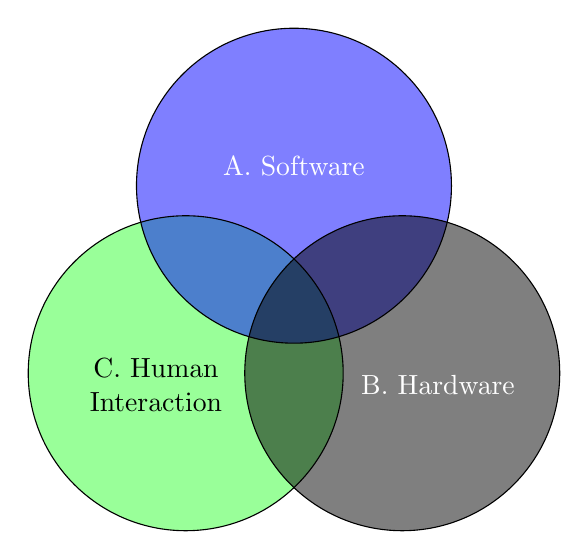
\begin{tikzpicture}
    \begin{scope}[shift={(3cm,-5cm)}, fill]
        \fill[green!80,opacity=0.5] \firstcircle;
        \fill[blue,opacity=0.5] \secondcircle;
        \fill[black,opacity=0.5] \thirdcircle;
        \draw \firstcircle node [yshift=-1ex,xshift=-2.5ex,align=center] {C. Human\\Interaction};
        \draw \secondcircle node [above,color=white] {A. Software};
        \draw \thirdcircle node [yshift=-1ex,xshift=3ex,color=white] {B. Hardware};
    \end{scope}
\end{tikzpicture}         
}
\caption{Research strands in mobile autonomy.}
 \label{fig:intro_autonomy_venn}
     \end{subfigure}
     \hfill
     \begin{subfigure}[b]{0.3\textwidth}
         \centering
\def\firstcircle{(0,0) circle (2cm)}
\def\secondcircle{(60:2.75cm) circle (2cm)}
\def\thirdcircle{(0:2.75cm) circle (2cm)}
\scalebox{0.75}{
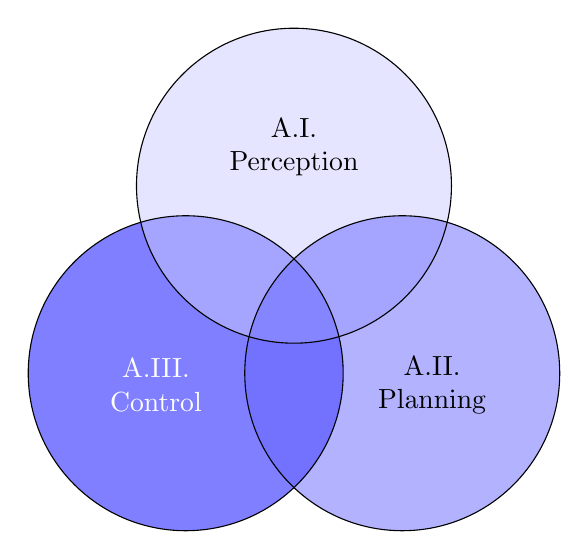
\begin{tikzpicture}
    \begin{scope}[shift={(3cm,-5cm)}, fill]
        \fill[blue,opacity=0.5] \firstcircle;
        \fill[blue!20,opacity=0.5] \secondcircle;
        \fill[blue!60,opacity=0.5] \thirdcircle;
        \draw \firstcircle node [align=center,yshift=-1ex,xshift=-2.5ex,color=white] {A.III.\\Control};
        \draw \secondcircle node [above,align=center,color=black] {A.I.\\Perception};
        \draw \thirdcircle node [align=center,yshift=-1ex,xshift=2.5ex] {A.II.\\ Planning};
    \end{scope}
\end{tikzpicture} 
}        \caption{The components of software research.}
         \label{fig:intro_software_venn}
 \end{subfigure}
 \hfill
      \begin{subfigure}[b]{0.3\textwidth}
         \centering
\def\firstcircle{(0,0) circle (2cm)}
\def\secondcircle{(60:2.75cm) circle (2cm)}
\def\thirdcircle{(0:2.75cm) circle (2cm)}
\scalebox{0.75}{
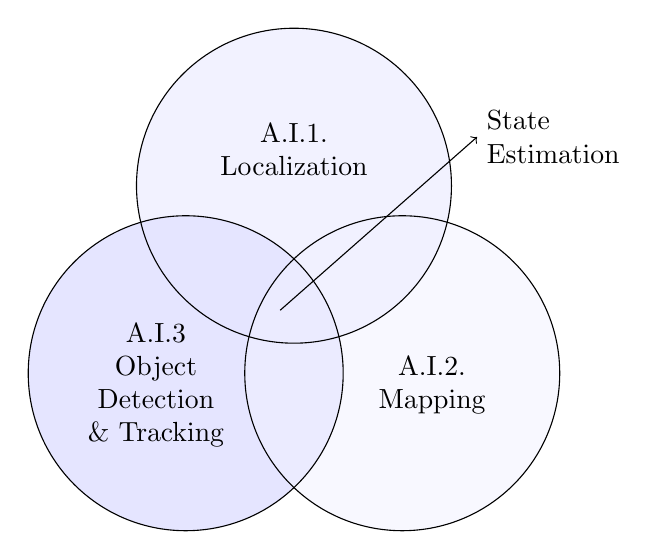
\begin{tikzpicture}
    \begin{scope}[shift={(3cm,-5cm)}, fill]
        \fill[blue!20,opacity=0.5] \firstcircle;
        \fill[blue!10,opacity=0.5] \secondcircle;
        \fill[blue!5,opacity=0.5] \thirdcircle;
        \draw \firstcircle node [align=center,yshift=-1ex,xshift=-2.5ex] {A.I.3\\Object\\Detection\\ \& Tracking};
        \draw \secondcircle node [above,align=center] {A.I.1.\\Localization};
        \draw \thirdcircle node [align=center,yshift=-1ex,xshift=2.5ex] {A.I.2.\\Mapping};
        \draw[->] (1.2,0.8) -- (3.7,3) node[right,align=left] {State\\Estimation};
    \end{scope}
\end{tikzpicture} 
}        \caption{The components of perception.}
         \label{fig:intro_perception_venn}
 \end{subfigure}
        \caption{Venn diagrams of modern mobile autonomy.}
        \label{fig:intro_three_venn}
\end{figure}


\section{The \textit{State} of State Estimation}


Central to many autonomous systems is the idea of a pipeline that processes high dimensional data and extracts some useful quantity. 

 of  the \textit{measurement model}, a mathematical entity that relates  observed measurement data to latent state parameters. By quantifying information contained within sensor data, probabilistic measurement models facilitate the construction of complex state estimation architectures that can fuse observations from sensors of varied modality to create rich models of the external world and infer the state of a mobile robot within it. My thesis focuses on egomotion estimation: the problem of accurately and consistently estimating the relative pose of a moving robot. For this task, a variety of different sensors may be useful (e.g., lidar, stereo cameras, or inertial measurement units), and each may allow for various hand-crafted or learned probabilistic measurement models.




For instance, modern visual and inertial egomotion estimation pipelines \citep{Leutenegger2015-fk, Cvisic2015-mt, Tsotsos2015-qs} have achieved impressive localization accuracy on trajectories spanning several kilometres by carefully extracting and tracking sparse visual features (using \textit{hand-crafted} algorithms) across consecutive images. Simultaneously, significant effort has gone to developing localization pipelines that eschew sparse features in favour of  \textit{dense} visual data \citep{Alcantarilla2016-kv, Forster2014-bm}, \todo{Add some modern citations here} typically relying on loss functions that use direct pixel intensities. Notably, in both the dense and sparse approaches, the visual observation model is often assumed to have an uncertainty model that is static, and known a priori.
\section{Classical Visual Estimation Pipelines}

\begin{figure}
\begin{center}
		\includegraphics[width=0.98\textwidth]{introduction/vo_pipeline.pdf}
		\caption{A traditional visual odometry pipeline.}
  	\label{fig:intro_vo_pipeline}
\end{center}
\end{figure}

\section{Pseudo Sensors}

\begin{figure}
\begin{center}
		\includegraphics[width=0.98\textwidth]{introduction/pseudo_sensor.pdf}
		\caption{A learned \textit{pseudo-sensor} extracts latent information from the same data stream.}
  	\label{fig:intro_pseudo_sensor}
\end{center}
\end{figure}


\section{Measurement Models}
A core component of any state estimation pipeline is the \textit{measurement model}, a mathematical entity that relates  observed measurement data to latent state parameters. By quantifying information contained within sensor data, probabilistic measurement models facilitate the construction of complex state estimation architectures that can fuse observations from sensors of varied modality to create rich models of the external world and infer the state of a mobile robot within it. My thesis focuses on egomotion estimation: the problem of accurately and consistently estimating the relative pose of a moving robot. For this task, a variety of different sensors may be useful (e.g., lidar, stereo cameras, or inertial measurement units), and each may allow for various hand-crafted or learned probabilistic measurement models.

For instance, modern visual and inertial egomotion estimation pipelines \citep{Leutenegger2015-fk, Cvisic2015-mt, Tsotsos2015-qs} have achieved impressive localization accuracy on trajectories spanning several kilometres by carefully extracting and tracking sparse visual features (using \textit{hand-crafted} algorithms) across consecutive images. Simultaneously, significant effort has gone to developing localization pipelines that eschew sparse features in favour of  \textit{dense} visual data \citep{Alcantarilla2016-kv, Forster2014-bm}, \todo{Add some modern citations here} typically relying on loss functions that use direct pixel intensities. Notably, in both the dense and sparse approaches, the visual observation model is often assumed to have an uncertainty model that is static, and known a priori. %here is a dearth of research towards building better uncertainty representations.

In the last several years, a significant part of the state estimation literature has focused on learned visual measurement models through convolutional neural networks (CNNs). Although initially developed for image classification  \citep{LeCun2015-qf}, CNN-based measurement models have been applied to numerous problems in geometric state estimation (e.g., homography estimation \citep{DeTone2016-ue}, single image depth reconstruction \citep{Garg2016-ip},  camera re-localization \citep{Kendall2016-zf}, place recognition \citep{Sunderhauf2015-is}). A number of recent CNN-based approaches have also tackled the problem of egomotion estimation, often purporting to obviate the need for classical visual localization pipelines by learning pose changes \textit{end-to-end}, directly from image data (e.g., \cite{Melekhov2017-dl}, \cite{Handa2016-hm}, \cite{Oliveira2017-lt}).

Despite this surge of excitement, significant debate has emerged within the robotics and computer vision communities regarding the extent to which deep models should replace existing geometric state estimation algorithms. Owing to their representational power, deep models may move the onerous task of selecting `good' (i.e., robust to environmental vagaries and sensor motion) visual features from the roboticist to the learned model. By design, deep models also provide a straight-forward formulation for using \textit{dense} data while being flexible in their loss function, and taking full advantage of modern computing architecture to minimize run time. Despite these potential benefits, current deep regression techniques for state estimation often generalize poorly to new environments, come with few analytical guarantees, and provide only point estimates of latent parameters.


\section{Outstanding Issues in the Field}

\subsection{The limits of homoscedastic noise models}

Although several state-of-the-art state estimation pipelines  \citep{Leutenegger2015-fk, Cvisic2015-mt} leave observation uncertainty associated with sensor measurements as a static tuning parameter, recent work \citep{Vega-Brown2014-sb, Hu2015-uw} suggests that using a stationary, homoscedastic noise in observation models can often reduce the consistency and accuracy of state estimates. This is especially true for complex, inferred measurement models. In foot-mounted navigation, the inferred zero velocity detector may be more or less informative depending on the exact type of motion and individual gait. In visual data, inferred visual observations can be degraded not only due to sensor imperfections (e.g. poor intrinsic calibration, digitization effects, motion blur), but also as a result of the observed environment (e.g. self-similar scenes, specular surfaces, textureless environments). Indeed, robust costs \cite{Alcantarilla2016-kv, MacTavish2015-wt, Agarwal2013-jq} and whiteness tests \citep{Tsotsos2015-qs} have commonly been used to alleviate the problem of poor noise modelling, but more work is required to better learn uncertainty in complex measurement models.


\subsection{Deep, learned models with no uncertainty estimates}
Although the paradigm of deep neural networks has resulted in several significant achievements in the fields of computer vision \citep{LeCun2015-qf}, these types of models have largely focused on point estimates (in either regression or classification) without any principled uncertainty estimates. Recently, the regularization techniques of dropout and dropconnect in Convolutional Neural Networks have been linked with approximate variational inference in homoscedastic Gaussian Processes \citep{Gal2015-bf, Kendall2016-zf, McClure2016-ai}, and the statistical technique of \textit{bootstrapping} has been applied to Deep Q Networks \citep{Osband2016-jg} to infer uncertainty, but both techniques are in their infancy. Recent work \citep{Osband_undated-wl} has also suggested that the former technique of dropout-based `uncertainty' is actually a measure of \textit{risk} (i.e., stochasticity in the measurements) and not \textit{uncertainty} over state parameters. Further, the same work showed that even this risk quantification can be arbitrarily bad given a fixed dropout parameter (which is typically the case).

\subsection{Integration of deep models into state estimation pipelines}
 To integrate the power of deep networks into state estimation algorithms, the recent literature differs in how to proceed. While some attempt to parametrize geometric transformations in their unconstrained state, and then learn the resulting state within a deep network regression optimization \citep{Costante2016-hb, Kendall2015-kh}, others integrate deep networks within outer estimation loops \citep{Haarnoja2016-ph}. Yet other work has used the neural network as an error correcting mechanism on top on an existing kinematic or dynamic model \citep{Punjani2015-pj}. This integration is made more difficult by the lack of uncertainty estimates associated with many learned measurement models in the computer vision and machine learning literature.
 
 
\section{Original Contributions}
The original contributions of my dissertation include three architectures that incorporate novel ways of using learned measurement models to improve egomotion estimation: PROBE, Sun-BCNN, and DPC-Net. Since the last D.E.C. meeting, I focussed on the latter two, and hope to build on DPC-Net in the final part of my thesis.

\subsection{Predictive Robust Estimation for Sparse Visual Odometry}

Predictive Robust Estimation (PROBE) is a technique that uses k-NN regression (original PROBE) or Generalized Kernels \citep{Vega-Brown2014-sb} (PROBE-GK) to train a predictive model for heteroscedastic measurement covariance to improve estimator accuracy and consistency. PROBE \citep{Peretroukhin2015-em} and PROBE-GK \citep{Peretroukhin2016-om} were published at IROS 2015 and ICRA 2016, respectively. For more information about PROBE, please refer to my past D.E.C. reports.

\subsection{Software Sun Sensor using a Bayesian Convolutional Neural Network}
Sun-BCNN is a technique to infer a probabilistic estimate of the direction of the sun from a single RGB image using a Bayesian Convolutional Neural Networks (BCNN). The method works much like dedicated sun sensors \citep{Lambert2012-sn}, but requires no additional hardware, and can provide mean and covariance estimates that can be readily incorporated into existing visual odometry frameworks. I worked on this project in collaboration with Lee Clement. While he focussed on integrating Sun-BCNN into the visual estimator, I developed the BCNN architecture and focused on uncertainty modelling. Initial exploratory work was published at ISER 2016, and the BCNN improvement was presented at ICRA 2017. An additional journal paper summarizing the work of the prior two papers, adding data from the Canadian High Arctic and Oxford, and investigating the effect of cloud cover and transfer learning was published in the International Journal of Robotics' Research, Special Issue on Experimental Robotics at the end of 2017.


%\begin{wrapfigure}{r}{0.5\textwidth}
%  \vspace{-40pt}
%  \begin{center}
%    \includegraphics[width=0.48\textwidth]{dpc_high_level.pdf}
%  \end{center}
%   \vspace{-10pt}
%  \caption{The DPC-Net system. Learned SE(3) pose corrections are fused with pose estimates from a classical estimator.}
%  	\label{fig:dpc_system}
%\end{wrapfigure}

\begin{figure}
\begin{center}
		\includegraphics[width=0.48\textwidth]{introduction/dpc_high_level.pdf}
		\caption{The DPC-Net system. Learned SE(3) pose corrections are fused with pose estimates from a classical estimator.}
  	\label{fig:dpc_system}
\end{center}

\end{figure}


\subsection{Deep Pose Corrections (DPC-Net)}
Deep Pose Correction (DPC, \Cref{fig:dpc_system}) is a novel approach to improving egomotion estimates through pose corrections learned through deep regression. DPC takes as its starting point an efficient, classical localization algorithm that computes high-rate pose estimates. To it, it adds a Deep Pose Correction Network (DPC-Net) that learns low-rate, `small' \textit{corrections} from training data that are then fused with the original estimates. DPC-Net does not require any modification to an existing localization pipeline, and can learn to correct multi-faceted errors from estimator bias, sensor mis-calibration or environmental effects. DPC-Net was accepted for publication in the proceedings of ICRA 2018, and as part of Robotics and Automation Letters \citep{2018_Peretroukhin_Deep}.

\subsection{Probabilistic $\LieGroupSE{3}$ inference using deep networks}

In the final part of my dissertation, I am investigating ways in which a network like DPC-Net can produce consistent probabilistic pose (i.e., SE(3)) estimates. By inferring a probability density over the unconstrained Lie algebra coordinates, one can induce a probability density over the group. There are several ways to proceed with the former induction.  Although I have already published work on Bayesian CNNs, as mentioned in the introduction, the validity of their uncertainty estimates has come into question. One potential alternative is to merge Gaussian Processes and deep networks through deep kernel learning \citep{Wilson2016-vy}. Although theoretically promising, this technique still scales poorly with training data size.

 Instead, I am investigating non-Bayesian approaches that learn a bespoke covariance matrix as part of their output using a log likelihood loss. By parametrizing the precision matrix through a Cholesky decomposition, it is possible to output positive definite matrices without enforcing any constraints on the network output (this approach was presented in the context of deep networks \citep{Haarnoja2016-ph}, and in the context of heteroscedastic noise modelling in \citep{Hu2015-uw}; it is similar in principal to switchable constraints \citep{Agarwal2013-jq}).
 
 Another potential alternative method is bootstrap aggregation (bagging). Bagging can be used to compute confidence bounds by training several models on randomly sub-sampled data (e.g., uncertainty for deep Q networks \citep{Osband2016-jg}). To reduce the cost of training multiple models, a number of authors have also suggested training a single network with multiple heads \citep{Lee2015-af}, \citep{Lakshminarayanan2016-zh}. I am investigating this latter approach, and also combining it with the log likelihood covariance learning.

